\chapter{JPEG}

\section{Overview}

JPEG, which stands for Joint Photographic Experts Group (the name of the committee that created the JPEG standard) is a lossy compression algorithm for images. A lossy compression scheme is a way to inexactly represent the data in the image, such that less memory is used yet the data appears to be very similar. This is why JPEG images look almost the same as the original images they were derived from most of the time unless the quality is reduced significantly, in which case there will be visible differences.

The JPEG algorithm takes advantage of the fact that humans can't see colors at high frequencies. These high frequencies are the data points in the image that are eliminated during the compression. JPEG compression also works best on images with smooth colour transitions.

JPEG is a commonly used method of lossy compression for digital
images. The degree of compression can be adjusted, allowing a
the tradeoff between storage size and image quality with a
compression ratio 10:1 but with little perceptible loss in image
quality.

\begin{figure}[!ht]
    \centering
    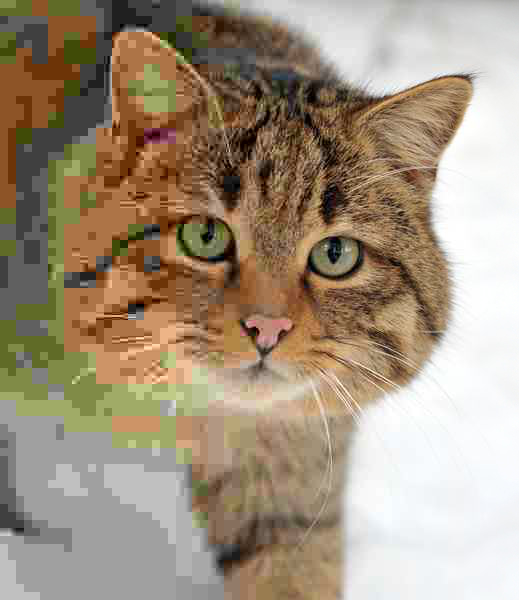
\includegraphics[width=0.40\textwidth]{fig/3-1.png}
    \captionsource{A photo of a European wildcat with the compression rate decreasing and hence quality increasing, from left to right.}
    {\url{https://en.wikipedia.org/wiki/JPEG}}
    \label{fig:jpegCompression}
\end{figure}

\vspace{2em}

\section{Algorithm}

\begin{figure}[!ht]
    \centering
    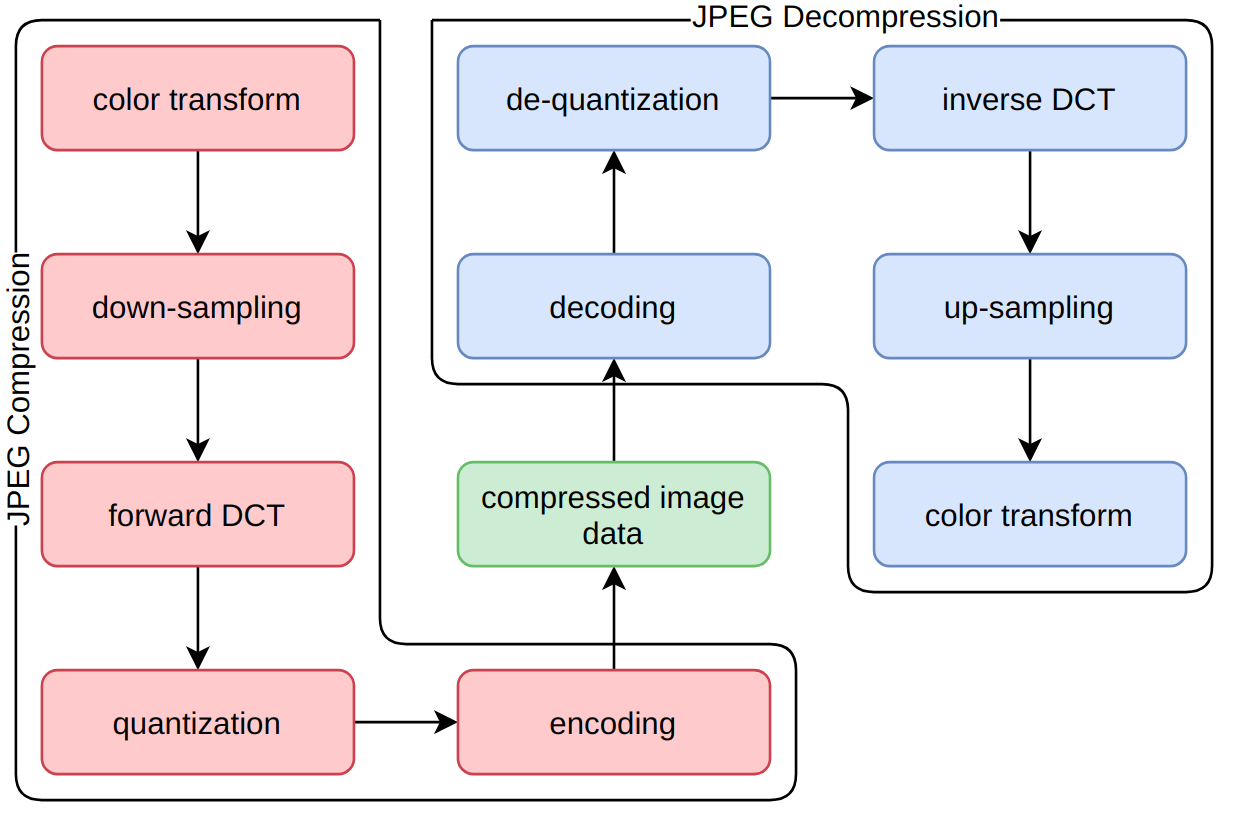
\includegraphics[width=0.80\textwidth]{fig/3-2.png}
    \caption{JPEG Schematic}
    \label{fig:jpegSchematic}
\end{figure}


\subsection{Splitting}

JPEG uses transform coding, it is largely based on the following observations:

\begin{itemize}
    \item Usually image contents change relatively slowly across images, i.e., it is unusual for intensity values to alter up and down several times in a small area, for example, within an $8 \times 8$ image block. A translation of this fact into the spatial frequency domain, implies, generally, lower spatial  frequency components contain more information than the high frequency components which often correspond to less useful details and noises.
    \item Experiments suggest that humans are more immune to loss of higher spatial frequency components than loss of lower frequency components. Human vision is insensitive to high frequency components.
\end{itemize}

Hence, first step is to split the image into $8 \times 8$ blocks non-overlapping pixel blocks. If the image cannot be divided into $8 \times 8$ blocks then the block is zero padded.

\vspace{1em}

\begin{figure}[!ht]
    \centering
    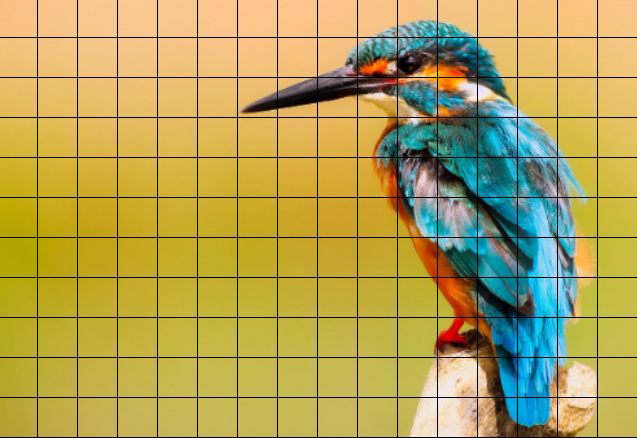
\includegraphics[width=0.50\textwidth]{fig/3-3.png}
    \caption{Splitting into $8 \times 8$ blocks}
    \label{fig:splitting}
\end{figure}

\subsection{Color Space Transform}

JPEG makes use of $[Y, Cb, Cr]$ model instead of $[R, G, B]$ model. There is a reason for using the color space. The human eye is more sensitive to luminance than to chrominance. 

\begingroup
\centering
    \begin{tabular}{|l|}
    \hline
    $Y = 0.299R + 0.587G + 0.114B$              \\ \hline
    $Cb = -0.1687R - 0.3313G + 0.5B + 128$      \\ \hline
    $Cr = 0.5R - 0.4187G - 0.0813B + 128$       \\ \hline
    $R = Y + 1.402 (Cr - 128)$                   \\ \hline
    $G = Y - 0.34414 (Cb - 128) - 0.71414(Cr - 128)$ \\ \hline
    $B = Y + 1.772  (Cb - 128)$                   \\ \hline
    \end{tabular}
\captionof{table}{RGB and YCbCr conversion table}\label{tbl:RGBYCbCrTable}
\endgroup


\subsection{Down-sampling}

After the color space transformation, the image is downsampled.
Downsampling happens in such a way that $Y$ is taken for each pixel whereas $Cb$ and $Cr$ is taken for $2 \times 2$ blocks.

Sometimes this steps is not carried out.

\subsection{Discrete Cosine Transform}

The key to the JPEG baseline compression process is a mathematical transformation known as the Discrete Cosine Transform (DCT). The DCT is in a class of mathematical operations that includes the well known Fast Fourier Transform (FFT), as well as many others. The basic purpose of these operations is to take a signal and transform it from one type of representation to another. For example, an image is a two-dimensional signal that is perceived by the human visual system. The DCT can be used to convert the signal (spatial information) into numeric data (“frequency” or “spectral” information) so that the image's information exists in a quantitative form that can be manipulated for compression.

The DCT is performed on an $N \times N$ square matrix of pixel values, and it yields an $N \times N$ square matrix of frequency coefficients. (In practice, N most often equals 8 because a larger block, though would probably give better compression, often takes a great deal of time to perform DCT calculations, creating an unreasonable tradeoff. As a result, DCT implementations typically break the image down into more manageable $8 \times 8$ blocks.) The DCT formula looks somewhat intimidating at first glance but can be implemented with a relatively straightforward piece of code.

\begin{equation}
    \begin{split}
    DCT[i,j] = \frac{1}{\sqrt{2N}} \: C[i] \: C[j] \; \sum_{x=0}^{N-1} \sum_{y=0}^{N-1} \; I[x,y] \: cos[\frac{(2x + 1)i\pi}{2N}] \: cos[\frac{(2y + 1)j\pi}{2N}]  \\
    where \; C(x) = \frac{1}{\sqrt{2}} \; if \; x=0, \; else \;1 \; if \; x>0
    \end{split}
\end{equation}

\vspace{2em}

\begin{equation}
    \begin{bmatrix}
        140 & 144 & 147 & 140 & 140 & 155 & 179 & 175\\ 
        144 & 152 & 140 & 147 & 140 & 148 & 167 & 179\\ 
        152 & 155 & 136 & 167 & 163 & 162 & 152 & 172\\ 
        168 & 145 & 156 & 160 & 152 & 155 & 136 & 160\\ 
        162 & 148 & 156 & 148 & 140 & 136 & 147 & 162\\ 
        147 & 167 & 140 & 155 & 155 & 140 & 136 & 162\\ 
        136 & 156 & 123 & 167 & 162 & 144 & 140 & 147\\ 
        148 & 155 & 136 & 155 & 152 & 147 & 147 & 136
    \end{bmatrix}   
\end{equation}

$\begin{bmatrix}
    140 & 144 & 147 & 140 & 140 & 155 & 179 & 175\\ 
    144 & 152 & 140 & 147 & 140 & 148 & 167 & 179\\ 
    152 & 155 & 136 & 167 & 163 & 162 & 152 & 172\\ 
    168 & 145 & 156 & 160 & 152 & 155 & 136 & 160\\ 
    162 & 148 & 156 & 148 & 140 & 136 & 147 & 162\\ 
    147 & 167 & 140 & 155 & 155 & 140 & 136 & 162\\ 
    136 & 156 & 123 & 167 & 162 & 144 & 140 & 147\\ 
    148 & 155 & 136 & 155 & 152 & 147 & 147 & 136
\end{bmatrix}$


\section{Conclusion}
In this chapter, we proposed a distributed algorithm
for construction of xyz.
The complexity of this algorithm is $O(n \log n)$.
Next chapter presents
another distributed algorithm which has linear time 
complexity based on xyz.

